\section{Wireframes}

  \subsection{Design choices}

    \begin{figure}[H]
      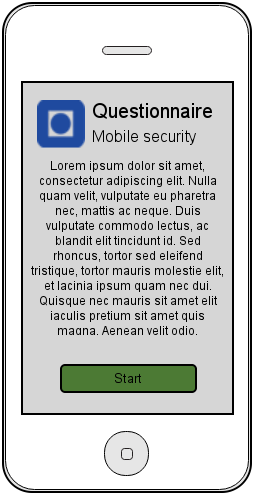
\includegraphics[scale=0.5]{screens/v2/mobile/mobile1-1.png}
    \end{figure}

    \begin{figure}[H]
      \centering
      \subfigure{
        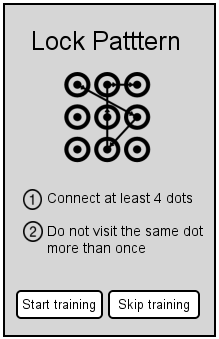
\includegraphics[scale=0.48]{screens/v2/plain/plain1-2.png}
      }
      \subfigure{
        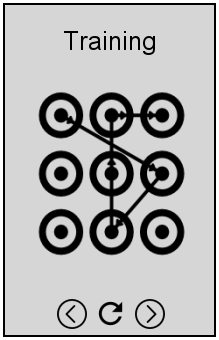
\includegraphics[scale=0.48]{screens/v2/plain/plain1-3.png}
      }
      \subfigure{
        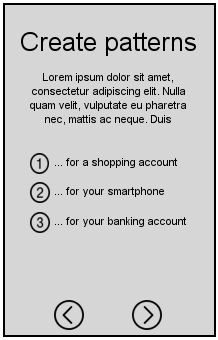
\includegraphics[scale=0.48]{screens/v2/plain/plain1-4.png}
      }
    \end{figure}

    \begin{figure}[H]
      \centering
      \subfigure{
        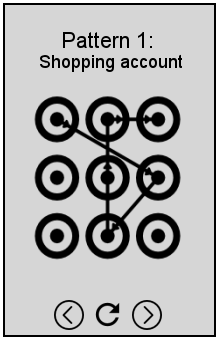
\includegraphics[scale=0.48]{screens/v2/plain/plain1-5.png}
      }
      \subfigure{
        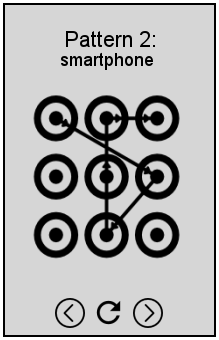
\includegraphics[scale=0.48]{screens/v2/plain/plain1-6.png}
      }
      \subfigure{
        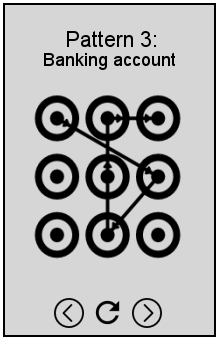
\includegraphics[scale=0.48]{screens/v2/plain/plain1-7.png}
      }
    \end{figure}

    \begin{figure}[H]
      \centering
      \subfigure{
        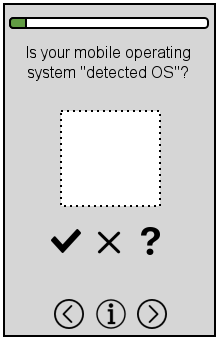
\includegraphics[scale=0.48]{screens/v2/plain/plain2-1.png}
      }
      \subfigure{
        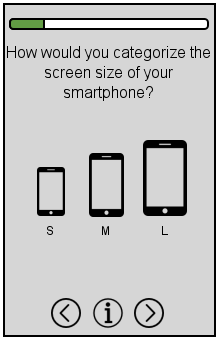
\includegraphics[scale=0.48]{screens/v2/plain/plain2-2.png}
      }
      \subfigure{
        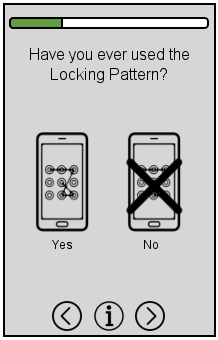
\includegraphics[scale=0.48]{screens/v2/plain/plain2-3.png}
      }
    \end{figure}

    \begin{figure}[H]
      \centering
      \subfigure{
        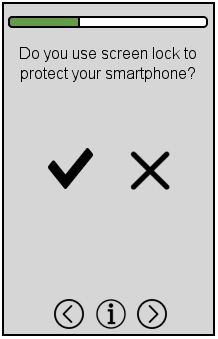
\includegraphics[scale=0.48]{screens/v2/plain/plain2-4.png}
      }
      \subfigure{
        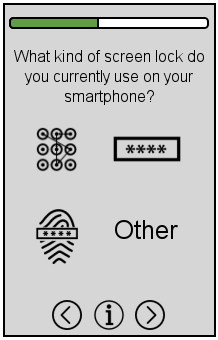
\includegraphics[scale=0.48]{screens/v2/plain/plain2-5.png}
      }
      \subfigure{
        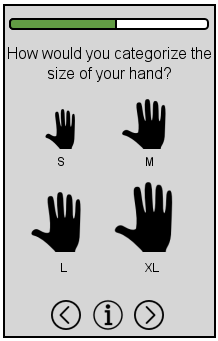
\includegraphics[scale=0.48]{screens/v2/plain/plain2-6.png}
      }
    \end{figure}

    \begin{figure}[H]
      \centering
      \subfigure{
        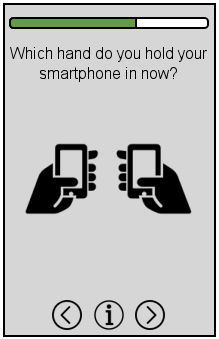
\includegraphics[scale=0.48]{screens/v2/plain/plain2-7.png}
      }
      \subfigure{
        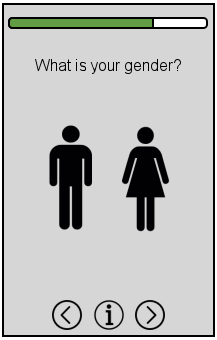
\includegraphics[scale=0.48]{screens/v2/plain/plain2-8.png}
      }
      \subfigure{
        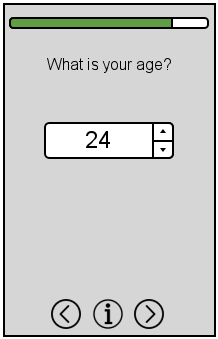
\includegraphics[scale=0.48]{screens/v2/plain/plain2-9.png}
      }
    \end{figure}

    \begin{figure}[H]
      \centering
      \subfigure{
        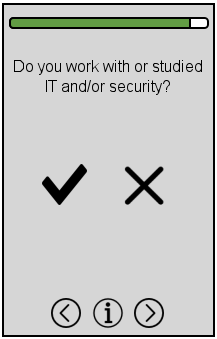
\includegraphics[scale=0.48]{screens/v2/plain/plain2-10.png}
      }
      \subfigure{
        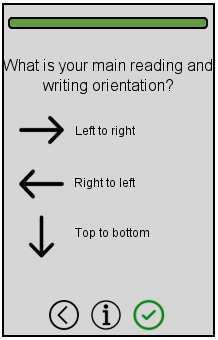
\includegraphics[scale=0.48]{screens/v2/plain/plain2-11.png}
      }
       \subfigure{
        
\includegraphics[scale=0.48]{screens/v2/plain/plain2-12.png}
      }
    \end{figure}

  \subsection{Pre-test and Pilot}\label{sec:pretest}
    When the questionnaire is ready, I need to perform a questionnaire to evaluate several aspects. First, I need to figure out if the respondents understand the questions stated in the questionnaire. This can cause a lot of bias in the data if the questions asked are ambiguous. Second, the time needed for completion of the questionnaire can not be too long. If the questionnaire takes too long to complete, there is less likely that people want to spend their time completing the questionnaire. It is stated that I need a sample size of 1000 for getting representative results for the analysis. At the same time, there is needed a lot of data to be able to make see patterns in the data. Therefore, it needs to be a balance between questions and data collected, and time of completion. 


    There is a need to do some quality testing before distributing the questionnaire over the Internet. A pen and paper test will be tested to check the wording of the questions as well as getting feedback of the amount of information that is asked for. It is also interesting to ask questions about the ethical aspects of the data collection. If some of the test persons feels that their privacy is leaked by answering the questionnaire, the questions might needs to be evaluated for the final questionnaire. 
    This test will also be conducted in the following spring when the system for data collection is up and running. 